\section{Introduction}

The SSD has increased significantly in density for the past decade. 
In 2011, a typical 2.5-inch SSD had 256GB capacity, but
%the world's first 2TB SSD was released in 2013~\cite{foremay2013}, but 
by 2018, a high-capacity SSD boasted a 30TB, expanding by 100× over the past ten years
~\cite{samsung2011, anandtech18samsung}. 
This remarkable growth of the device-capacity is thanks to the advanced scaling technologies 
such as nanoscale fabrication~\cite{busche2014design} and multi-layer stacking~\cite{9365809}. 
% such as nanoscale fabrication~\cite{busche2014design} and multi-layer stacking. 

% Unfortunately, not all components of the SSDs have kept up with the scaling rate.
% The capacitor, which is adopted in enterprise-class SSDs for power-loss protection (PLP), fails to proceed at the pace. Historically, storage devices 
% have been equipped with a small size of volatile buffer in front of the persistent disk. 
% By using them as a read cache and a write buffer, they hide a long latency of the physical storage medium 
% as well as mitigating an endurance limitation of the worn-out devices. 
% However, the volatile buffer loses all data in the event of power crash. 
% To prevent a data loss or corruption by this, enterprise-class SSDs
% rely on the capacitors; it reserves energy to persist data in volatile buffer 
% in the unforeseen event of a power crash. 
% In addition, the adoption of capacitors enables an SSD to ignore the \texttt{FLUSH} command that explicitly requests all data in the volatile buffer to be made durable.
% This property increases the buffering effect in SSD significantly, leading to both less write traffic and a shorter operation latency.

% \EUNJI{Historically, storage devices 
% have been equipped with a small size of volatile buffer in front of the persistent disk. 
% By using them as a read cache and a write buffer, they hide a long latency of the physical storage medium 
% as well as mitigating an endurance limitation of the worn-out devices.}
\iffalse
Unfortunately, the growth in SSD capacity is reaching its limit due to the stunted growth of \textit{capacitors}. 
\fi
The enterprise-class SSDs adopt the capacitor to protect data for volatile buffer in case of power crash. 
SSD-internal buffer is used for buffering user writes and caching translation information (also known as mapping table). 
If they are not protected, SSDs will have not only a data loss and/or corruption but also a long recovery time to build an up-to-date  mapping table by scanning entire flash drives.
To prevent this unwanted situation, enterprise-class SSDs
rely on the capacitors that persist data of the volatile buffer in a power loss using a reserved energy.

% In addition, the adoption of capacitors enables an SSD to ignore the \texttt{FLUSH} command that explicitly requests all data in the volatile buffer to be made durable.
% This property increases the buffering effect in SSD significantly, leading to both less write traffic and a shorter operation latency.

% The SSD-internal volatile buffer loses all data in the event of power crash. 
% To prevent a data loss or corruption by this, enterprise-class SSDs
% rely on the capacitors; it reserves energy to persist data in volatile buffer 
% in the unforeseen event of a power crash.
% In addition, the adoption of capacitors enables an SSD to ignore the \texttt{FLUSH} command that explicitly requests all data in the volatile buffer to be made durable.
% This property increases the buffering effect in SSD significantly, leading to both less write traffic and a shorter operation latency.

% To overcome this limitation without sacrificing performance, 
However, the reliance on capacitors is no longer sustainable as the increase in SSD far outpaces 
the increase in capacitor density. 
% the improvement in capacitance fails to keep up with the rapid growth of SSDs. 
%Al(aluminum) and Ta(tantalum)-electrolytic capacitors used in SSDs have increased in density through miniaturization by tenfold from 1960 to 2005 [4]. 
% Although the capacitance density has also steadily improved, 
% it is not as rapid as the SSD scaling speed. 
Al(aluminum) and Ta(tantalum)-electrolytic capacitors used in SSDs 
have increased in density by tenfold from 1960 to 2005. 
This is approximately 50x slower than the SSD density increase rate.
Because the internal buffer size increases in proportion to the storage capacity (typically 0.1\% of storage capacity~\cite{samsung_ratio, ni2017hash}),
the density gap between capacitance and memory technologies 
imposes an intrinsic limitation on the current architecture wherein 
the entire buffer is fully protected by capacitors. 

% \begin{figure}[t]
%     \centering{}
%     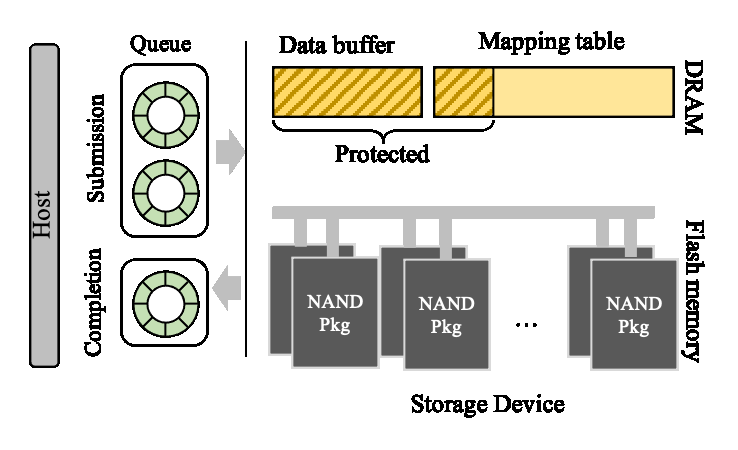
\includegraphics[width=0.4\textwidth]{figure/dawid_ssd_archi.eps}
%     %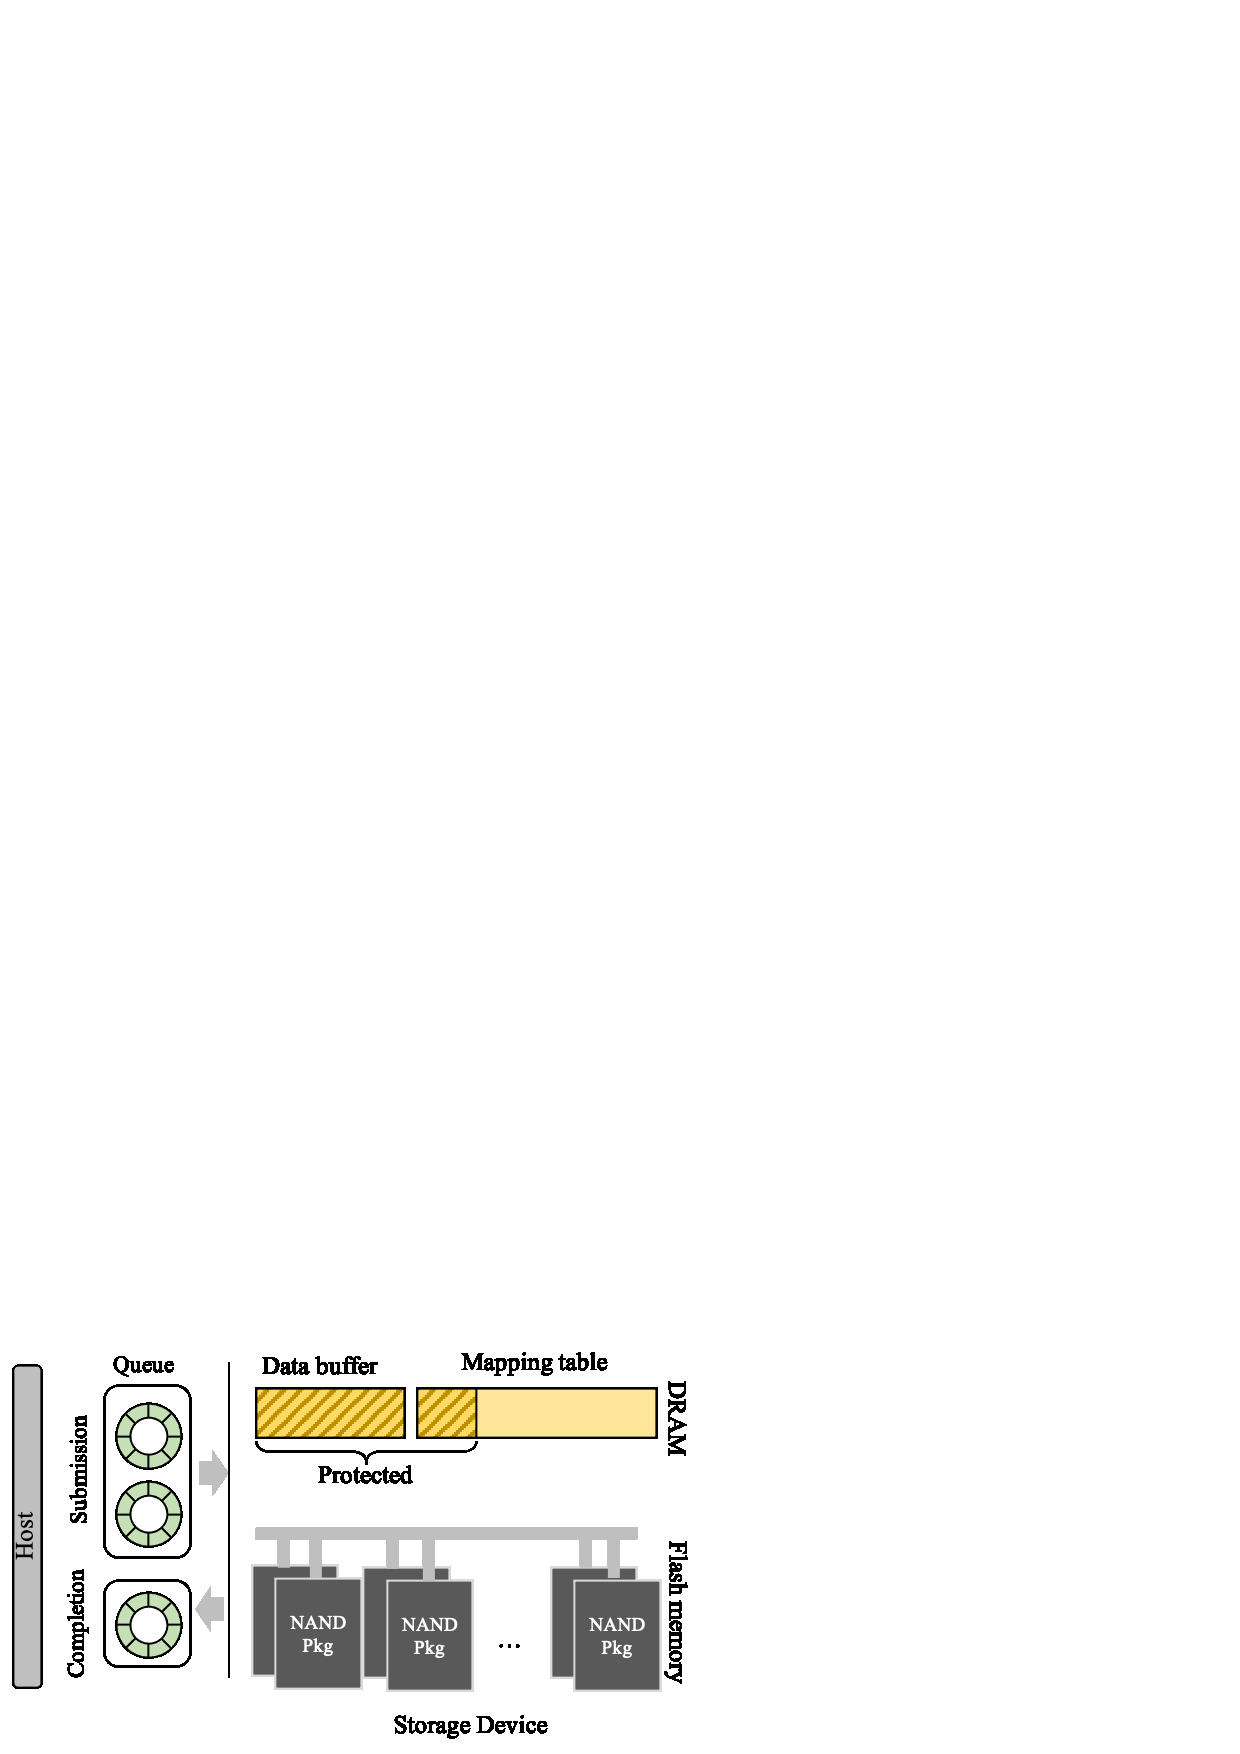
\includegraphics[width=0.4\textwidth]{figure/dawid_ssd_archi.png}
%     \caption{\textbf{SSD architecture with \ours{} buffer.}}
%     \label{fig_dawid_archi}
% \end{figure}
% \EUNJI{to scale ...}
This paper presents a device-internal buffer architecture called \ours{}
for the SSDs under capacitance constraints. 

\begin{itemize}
    \item Eviction policy : 맵핑 테이블의 일부만 보호되고 있을 때 보호범위를 넘어서면 더티 엔트리를 플러쉬 해야 함. 
    \item Re-ordering policy 
    \item Flush policy 
\end{itemize}

% which operates under capacitance constraints.
% Fig.~\ref{fig_dawid_archi} shows the SSD architecture targeted in our study. 


\textcolor{red}{
The data maintained in the buffer can be classified into two types: the actual user data and 
the metadata for SSD management (i.e, mapping table). 
When the buffer is partially protected, the number of dirty pages is limited to 
the maximum amount of data that the on-board capacitance can protect. 
If the number of dirty pages goes beyond the limit, changes should be flushed to the flash memory immediately
to meet the durability constraint for SSDs. 
}
